\newcolumntype{C}[1]{>{\centering\arraybackslash}m{#1}}
\chapter{Analyse et spécification des besoins} 
\minitoc
\newpage

\section{Introduction}
Dans le chapitre précédent, nous avons analysé le contexte général de notre projet en identifiant les problématiques auxquelles font face les professionnels du sport, et nous avons défini le cadre méthodologique Agile Scrum. Dans ce deuxième chapitre, nous entrons au cœur de l'ingénierie logicielle. Nous allons d’abord identifier avec précision les différents acteurs de notre système, pour ensuite dégager de manière exhaustive les besoins fonctionnels et non fonctionnels de notre projet. Ces besoins seront traduits sous la forme d'un Product Backlog priorisé. Ensuite, nous procéderons à une modélisation poussée via le diagramme de cas d'utilisation global et son dictionnaire détaillé. Enfin, nous justifierons nos choix technologiques et détaillerons l'architecture globale (physique et logique) de "CoachingApp".

\section{Spécification des besoins}
La spécification des exigences du projet consiste à traduire les objectifs de haut niveau du projet en un ensemble de fonctionnalités ciblées, compréhensibles à la fois par les développeurs et par les utilisateurs finaux.

\subsection{Identification des acteurs}
Un acteur représente l'abstraction d'un rôle joué par des entités externes (utilisateurs humains ou dispositifs matériels/logiciels) qui interagissent directement avec le système étudié. Pour CoachingApp, nous distinguons trois acteurs principaux, disposant chacun de droits d'accès spécifiques :
\begin{itemize}
    \item \textbf{L’Administrateur :} Ce profil dispose de privilèges absolus sur l'application. Il interagit exclusivement via le tableau de bord web (Angular). Son rôle est d'assurer la gouvernance de la plateforme. Il gère les comptes (bannissement, réactivation), surveille les KPIs (Key Performance Indicators) financiers et d'usage, et surtout, il maintient la bibliothèque globale des exercices (afin d'éviter que chaque coach ne crée des doublons dans la base de données).
    \item \textbf{Le Coach (ou Nutritionniste) :} C'est l'utilisateur cœur de cible professionnel de la plateforme. Il possède un profil public permettant aux athlètes de lui envoyer des requêtes de coaching. Une fois la relation validée, le coach accède à des outils avancés : création de programmes d'entraînement sur-mesure (structurés en macro-cycles et micro-cycles), assignation de régimes nutritionnels précis (macros), suivi de la progression de l'athlète via des graphiques interactifs, et communication continue.
    \item \textbf{L’Athlète :} Il s'agit de l'utilisateur final (le client du coach). L'athlète interagit principalement via l'application mobile (Flutter) conçue pour une utilisation nomade (notamment en salle de sport). Ses interactions comprennent la complétion de son profil biométrique (poids, taille, objectifs), la consultation de son planning quotidien, l'exécution interactive des séances via le Workout Player (avec chronomètres automatiques et saisie de la charge soulevée), le suivi de son journal alimentaire (DietLog), et la messagerie.
\end{itemize}

\subsection{Besoins fonctionnels}
Les besoins fonctionnels décrivent précisément les actions que le système doit être en mesure d'exécuter. Ils découlent directement de la problématique énoncée.

\subsubsection{Besoins de l'Administrateur}
\begin{itemize}
    \item S'authentifier de manière sécurisée sur l'interface d'administration Web.
    \item Consulter un tableau de bord analytique présentant des métriques temps réel (utilisateurs en ligne, nombre de programmes créés, etc.).
    \item Ajouter, modifier ou supprimer des exercices (Nom, Description, Groupe Musculaire Ciblé, Lien vidéo) dans la bibliothèque centrale.
    \item Bloquer ou supprimer un compte utilisateur enfreignant les conditions d'utilisation.
\end{itemize}

\subsubsection{Besoins du Coach}
\begin{itemize}
    \item Créer un compte professionnel et configurer son profil public (Spécialités, Tarifs, Expérience).
    \item Consulter la liste des "Coaching Requests" envoyées par des athlètes et les accepter/refuser.
    \item Construire des programmes d'entraînement hiérarchisés : Programme global $\rightarrow$ Jours spécifiques $\rightarrow$ Exercices avec paramètres (Séries, Répétitions, RPE, Temps de repos).
    \item Assigner un ou plusieurs programmes à un ou plusieurs athlètes de son répertoire.
    \item Fixer des objectifs macro-nutritionnels quotidiens (Protéines, Glucides, Lipides, Calories totales).
    \item Surveiller la conformité de l'athlète via des historiques d'entraînement et de repas.
    \item Échanger des messages textuels ou vocaux en temps réel avec ses clients.
\end{itemize}

\subsubsection{Besoins de l'Athlète}
\begin{itemize}
    \item S'inscrire, se connecter et remplir un formulaire d'intégration (Onboarding) capturant ses mesures corporelles et son objectif principal (ex: Hypertrophie).
    \item Rechercher un coach via un système de filtrage et envoyer une demande d'accompagnement.
    \item Visualiser son emploi du temps d'entraînement de la semaine.
    \item \textbf{Besoins critiques du lecteur interactif (Workout Player) :} Lancer une séance, lancer automatiquement le minuteur de repos après avoir coché une série, saisir le poids soulevé pour assurer la surcharge progressive.
    \item Renseigner ses repas quotidiens en ajoutant des aliments pour obtenir un calcul immédiat des macronutriments consommés.
    \item Recevoir des notifications push lors de la réception d'un message ou de l'assignation d'un nouveau programme.
\end{itemize}

\subsection{Besoins non fonctionnels}
Les besoins non fonctionnels définissent les critères de qualité globale, de sécurité et de performance que notre solution logicielle doit impérativement respecter.
\begin{itemize}
    \item \textbf{Ergonomie et Expérience Utilisateur (UX) :} L'application mobile (particulièrement le Workout Player) sera utilisée dans un environnement physique exigeant (salle de sport). L'interface doit comporter de gros boutons, un contraste élevé (Dark Mode de préférence), et minimiser les saisies textuelles lors de l'effort physique.
    \item \textbf{Sécurité et Confidentialité :} L’application traitant des données de santé personnelles, une sécurité stricte est requise. Les mots de passe doivent être hachés (algorithme bcrypt) avant stockage. L'authentification des requêtes HTTP doit utiliser des jetons \textbf{JWT (JSON Web Tokens)} signés avec expiration.
    \item \textbf{Performance et Temps Réel :} Le module de messagerie et la mise à jour des statistiques nécessitent une architecture temps réel (WebSockets) garantissant une latence inférieure à 200 ms pour l'envoi d'un message. Le chargement d'un programme lourd ne doit pas bloquer le thread principal du téléphone.
    \item \textbf{Disponibilité et Portabilité :} L'application mobile doit être cross-platform (iOS et Android) avec un comportement natif. L'API doit être disponible 24/7 pour permettre aux athlètes s'entraînant la nuit de synchroniser leurs données.
\end{itemize}

\section{Product Backlog}
Le Product Backlog correspond à une liste priorisée des besoins et des exigences. Nous avons utilisé la technique « MoSCoW » (Must have, Should have, Could have, Won't have) pour prioriser ces fonctionnalités. Les "Must" constituent le MVP (Minimum Viable Product).

\begin{table}[H]
\centering
\renewcommand{\arraystretch}{1.5}
\resizebox{\textwidth}{!}{%
\begin{tabular}{|>{\centering\arraybackslash}p{1.2cm}|p{3cm}|>{\centering\arraybackslash}p{1cm}|p{2cm}|p{7cm}|>{\centering\arraybackslash}p{1.5cm}|}
\hline
\rowcolor[HTML]{EFEFEF} 
\textbf{Sprint} & \textbf{Épopée (Epic)} & \textbf{ID} & \textbf{Acteur} & \textbf{User Story} & \textbf{Priorité} \\ \hline
1 & \multirow{3}{3cm}{Fondations \& Authentification}
& 1.1 & Tous & ETQ utilisateur, je veux créer un compte sécurisé pour accéder à l'application. & Must \\ \cline{3-6}
& & 1.2 & Athlète & ETQ athlète, je veux compléter mon profil biométrique pour cibler mes objectifs. & Must \\ \cline{3-6}
& & 1.3 & Coach/Athlète & ETQ utilisateur, je veux envoyer et accepter des demandes de coaching. & Must \\ \hline
2 & \multirow{3}{3cm}{Entraînement \& Nutrition (Cœur Métier)}
& 2.1 & Coach & ETQ coach, je veux construire un programme d'entraînement complexe avec plusieurs jours. & Must \\ \cline{3-6}
& & 2.2 & Athlète & ETQ athlète, je veux jouer ma séance avec un chronomètre intégré et valider mes séries. & Must \\ \cline{3-6}
& & 2.3 & Athlète & ETQ athlète, je veux enregistrer mes repas pour suivre mes macros quotidiens. & Should \\ \hline
3 & \multirow{3}{3cm}{Communication, IA \& Dashboard Admin}
& 3.1 & Tous & ETQ utilisateur, je veux communiquer instantanément avec mon interlocuteur via un chat intégré. & Should \\ \cline{3-6}
& & 3.2 & Admin & ETQ administrateur, je veux visualiser les métriques de la plateforme sur une interface web. & Should \\ \cline{3-6}
& & 3.3 & Coach & ETQ coach, je veux générer des variantes d'exercices à l'aide d'une Intelligence Artificielle. & Could \\ \hline
4 & \multirow{2}{3cm}{Métriques de Santé \& IoT}
& 4.1 & Athlète & ETQ athlète, je veux enregistrer mes mensurations corporelles historiques. & Should \\ \cline{3-6}
& & 4.2 & Athlète & ETQ athlète, je veux synchroniser mes pas et mon sommeil avec Google Fit/Apple Health. & Could \\ \hline
5 & \multirow{3}{3cm}{Visioconférence \& Agendas}
& 5.1 & Coach & ETQ coach, je veux définir mes plages de disponibilité sur mon calendrier. & Could \\ \cline{3-6}
& & 5.2 & Athlète & ETQ athlète, je veux planifier et réserver un rendez-vous avec mon coach. & Could \\ \cline{3-6}
& & 5.3 & Tous & ETQ utilisateur, je veux lancer un appel vidéo chiffré en direct. & Could \\ \hline
\end{tabular}%
}
\caption{Product Backlog détaillé et priorisé pour les 5 Sprints (Méthode MoSCoW)}
\end{table}

\section{Modélisation fonctionnelle avec UML}
\subsection{Diagramme de cas d’utilisation global}
Le diagramme de cas d’utilisation est essentiel pour capturer les exigences fonctionnelles du système du point de vue de l'utilisateur. Il décrit \textit{ce que} le système fait, sans se soucier de \textit{comment} il le fait. 

La figure 2.1 ci-dessous modélise l'ensemble des interactions majeures entre nos trois acteurs et la frontière du système CoachingApp.

\begin{figure}[H]
\centering
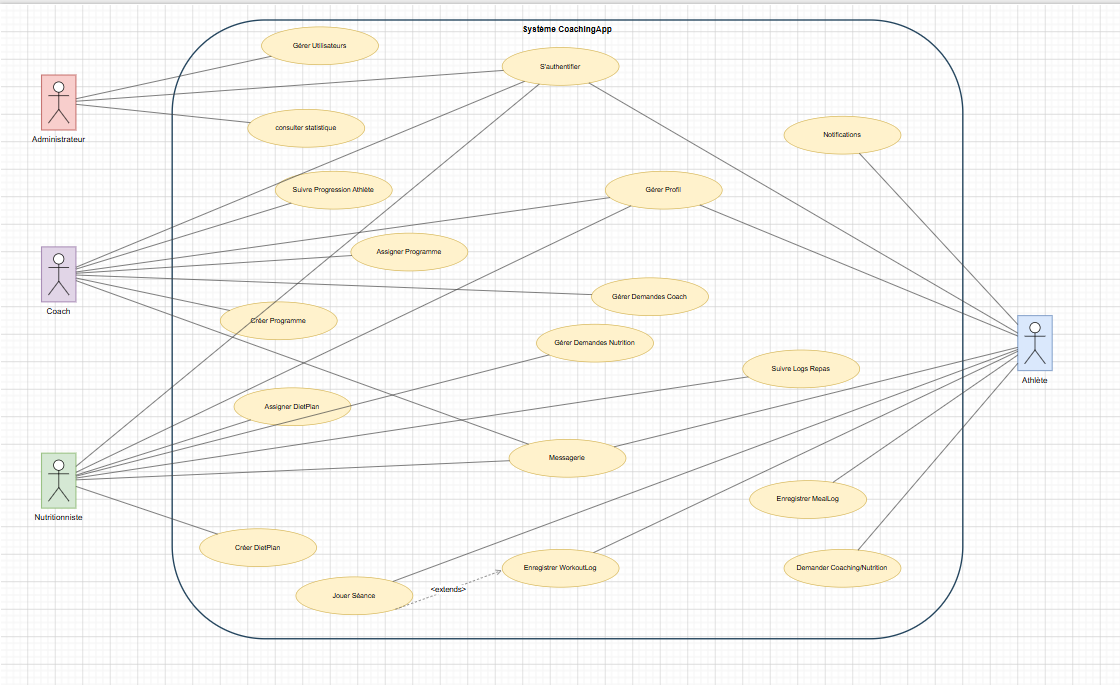
\includegraphics[width=0.9\textwidth]{diagrams/use case global.png}
\caption{Diagramme des cas d'utilisation global}
\end{figure}

\subsection{Dictionnaire des cas d'utilisation (Scénarios Détaillés)}
Afin de lever toute ambiguïté sur le comportement attendu du système lors des processus critiques, nous proposons le dictionnaire détaillé des cas d'utilisation majeurs.

\subsubsection{Cas 1 : S'authentifier}
\begin{table}[H]
\centering
\renewcommand{\arraystretch}{1.3}
\begin{tabular}{|p{4cm}|p{11cm}|}
\hline
\rowcolor[HTML]{EFEFEF} 
\textbf{Attribut} & \textbf{Description} \\ \hline
\textbf{Titre} & S'authentifier \\ \hline
\textbf{Acteur Principal} & Utilisateur (Coach, Athlète, ou Admin) \\ \hline
\textbf{Objectif} & Accéder à son espace personnel sécurisé \\ \hline
\textbf{Pré-conditions} & Posséder un compte valide enregistré dans la base de données \\ \hline
\textbf{Scénario nominal} & 
1. L'utilisateur ouvre l'application et saisit son email et son mot de passe.\newline
2. L'application envoie une requête de connexion à l'API.\newline
3. Le système vérifie les identifiants (comparaison du hash bcrypt).\newline
4. Le système génère un token JWT.\newline
5. L'utilisateur est redirigé vers son tableau de bord approprié. \\ \hline
\textbf{Scénarios alternatifs} & 
\textit{Identifiants erronés :} Le système affiche un message d'erreur et invite l'utilisateur à réessayer. \\ \hline
\end{tabular}
\end{table}

\subsubsection{Cas 2 : Créer un Programme d'Entraînement}
\begin{table}[H]
\centering
\renewcommand{\arraystretch}{1.3}
\begin{tabular}{|p{4cm}|p{11cm}|}
\hline
\rowcolor[HTML]{EFEFEF} 
\textbf{Attribut} & \textbf{Description} \\ \hline
\textbf{Titre} & Créer un Programme d'Entraînement \\ \hline
\textbf{Acteur Principal} & Coach \\ \hline
\textbf{Objectif} & Concevoir une routine sportive complète pour l'assigner à des athlètes \\ \hline
\textbf{Pré-conditions} & Être authentifié en tant que Coach \\ \hline
\textbf{Scénario nominal} & 
1. Le coach clique sur "Nouveau Programme".\newline
2. Il saisit le titre, la description et les objectifs du programme.\newline
3. Il ajoute des "Jours" d'entraînement (ex: Jour 1 - Push, Jour 2 - Pull).\newline
4. Pour chaque jour, il ajoute des exercices depuis le catalogue global.\newline
5. Il définit les séries, les répétitions, le poids cible et le repos pour chaque exercice.\newline
6. Le système valide et sauvegarde la structure hiérarchique complexe dans la base de données. \\ \hline
\end{tabular}
\end{table}

\subsubsection{Cas 3 : Exécuter une Séance (Workout Player)}
\begin{table}[H]
\centering
\renewcommand{\arraystretch}{1.3}
\begin{tabular}{|p{4cm}|p{11cm}|}
\hline
\rowcolor[HTML]{EFEFEF} 
\textbf{Attribut} & \textbf{Description} \\ \hline
\textbf{Titre} & Exécuter une Séance d'entraînement \\ \hline
\textbf{Acteur Principal} & Athlète \\ \hline
\textbf{Objectif} & Suivre son programme en temps réel à la salle de sport \\ \hline
\textbf{Pré-conditions} & Avoir un programme assigné par son coach pour le jour J \\ \hline
\textbf{Scénario nominal} & 
1. L'athlète clique sur "Démarrer la séance".\newline
2. L'interface plein écran affiche le premier exercice.\newline
3. L'athlète effectue sa série, saisit le poids réel soulevé et appuie sur "Valider".\newline
4. Le système démarre automatiquement le chronomètre de repos imposé par le coach.\newline
5. L'opération se répète jusqu'à la fin de la séance.\newline
6. Le système compile un rapport d'entraînement (WorkoutLog) et l'envoie au serveur. \\ \hline
\end{tabular}
\end{table}

\section{Justification des choix technologiques}
Avant de décrire l'architecture de notre système, il est indispensable de justifier la pile technologique (Tech Stack) retenue. Dans un écosystème logiciel en constante évolution, nos choix se sont orientés vers des technologies modernes, maintenables, et bénéficiant de communautés open-source massives.

\subsection{Côté Client (Frontend Mobile \& Web)}
\textbf{1. Flutter (Application Mobile Athlète/Coach)}
Flutter, le framework open-source créé par Google, s'est imposé comme une évidence pour notre interface mobile.
\begin{itemize}
    \item \textbf{Développement Cross-Platform :} Avec une seule base de code en langage \textit{Dart}, nous générons des applications natives pour iOS et Android, divisant ainsi le temps de développement par deux sans sacrifier les performances.
    \item \textbf{Performances proches du natif :} Contrairement à React Native qui utilise un pont JavaScript, Flutter compile directement en code machine ARM. Son moteur de rendu Skia permet des animations ultra-fluides (60fps), ce qui est crucial pour le bon fonctionnement du "Workout Player" chronométré.
\end{itemize}

\textbf{2. Angular (Tableau de bord Administrateur)}
Pour l'interface d'administration s'exécutant sur des navigateurs web desktop, nous avons choisi Angular (développé par Google).
\begin{itemize}
    \item \textbf{Architecture robuste :} Angular impose une structuration stricte par composants, services et modules, idéale pour une interface d'administration complexe (tableaux de données lourds, graphiques).
    \item \textbf{TypeScript natif :} L'utilisation de TypeScript garantit un typage fort, prévenant d'innombrables erreurs lors de la phase de compilation.
\end{itemize}

\subsection{Côté Serveur (Backend \& API)}
\textbf{3. Node.js et Express.js (Serveur d'application)}
Node.js permet d'exécuter du JavaScript côté serveur.
\begin{itemize}
    \item \textbf{Event-Driven \& Asynchrone :} Son architecture non bloquante est parfaite pour une application "I/O intensive" comme la nôtre, où le serveur doit interroger la base de données des milliers de fois pour récupérer des programmes et des logs sans bloquer les autres utilisateurs.
    \item \textbf{Express.js :} Ce micro-framework offre une syntaxe minimaliste pour créer des routes d'API RESTful claires et d'intégrer facilement des middlewares (comme la validation JWT).
\end{itemize}

\textbf{4. Socket.io (Communication Temps Réel)}
Pour le module de messagerie, les requêtes HTTP traditionnelles sont inadéquates (trop de latence). Socket.io établit une connexion bidirectionnelle persistante (WebSockets) entre le téléphone et le serveur Node.js, permettant aux messages d'arriver instantanément.

\subsection{Base de données et ORM}
\textbf{5. PostgreSQL (SGBD Relationnel)}
Bien que les bases NoSQL (comme MongoDB) soient populaires, la nature de nos données dictait le choix du relationnel. Un programme est lié à des jours, qui sont liés à des exercices de bibliothèque, qui génèrent des logs d'entraînement liés à un athlète précis. PostgreSQL, reconnu comme le SGBD open-source le plus avancé au monde, garantit la forte intégrité de ces données complexes.

\textbf{6. TypeORM (Mapping Objet-Relationnel)}
Au lieu d'écrire des requêtes SQL brutes sujettes aux erreurs, nous utilisons TypeORM côté backend. Il permet de manipuler les tables de la base de données comme de véritables classes TypeScript, automatisant la génération des clés étrangères et sécurisant l'application contre les injections SQL de manière native.

\section{Architecture du système}
L’architecture définit la manière dont les différentes composantes technologiques évoquées précédemment sont structurées et interagissent pour former une solution cohérente, résiliente et évolutive.

\subsection{Architecture physique (3-Tiers)}
Pour assurer la séparation des préoccupations (Separation of Concerns), notre plateforme adopte une architecture dite à "Trois Tiers" (Three-Tier Architecture), qui sépare physiquement l'interface utilisateur, la logique métier et le stockage des données.

\begin{figure}[H]
\centering
%[À FAIRE : Optionnel - Vous pouvez générer un diagramme d'architecture 3 tiers]
%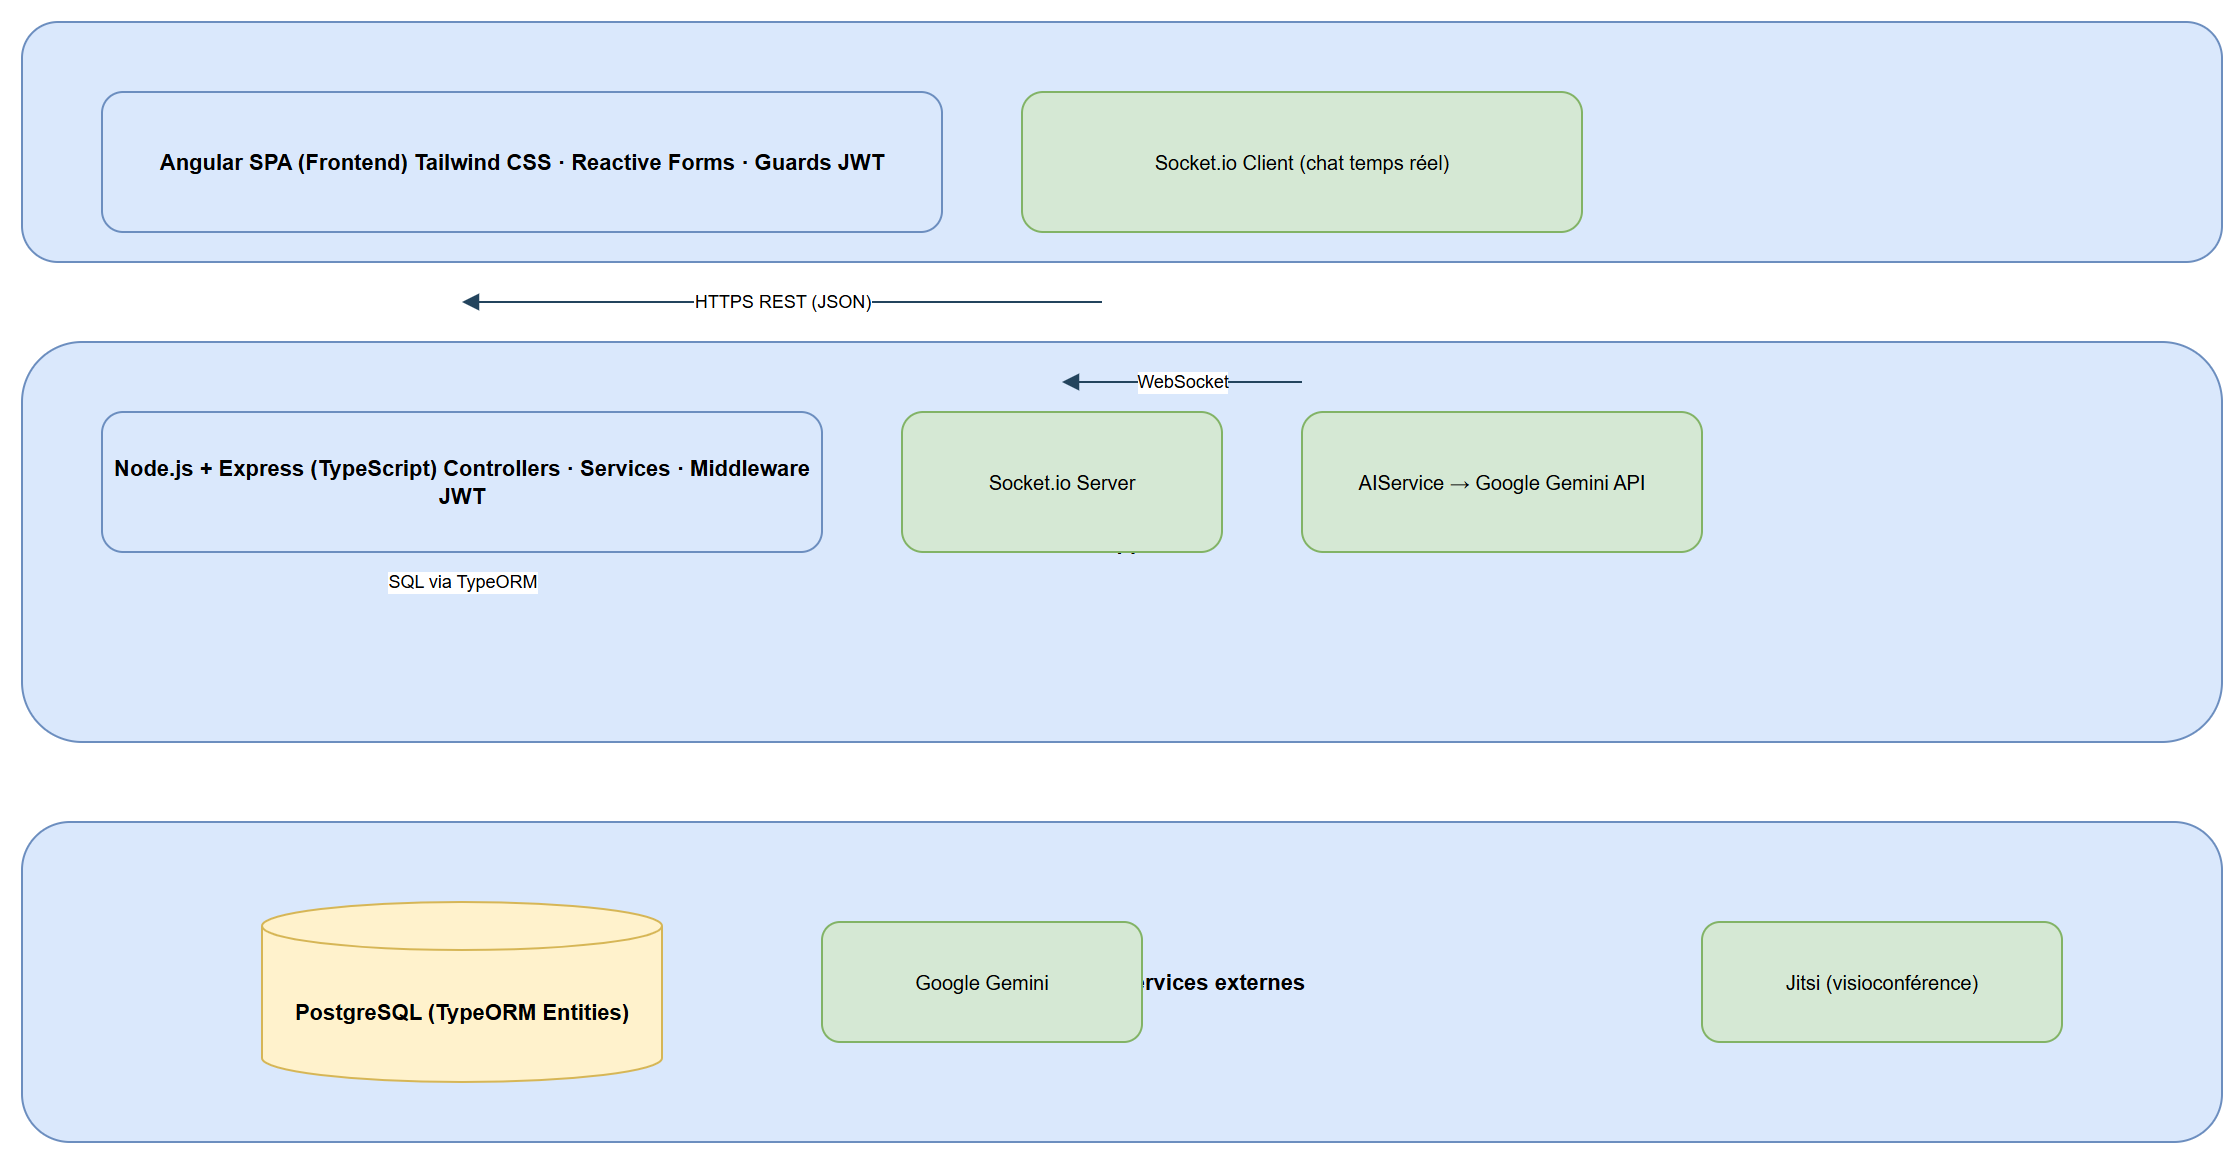
\includegraphics[width=0.8\textwidth]{diagrams/architecture_3_tiers.png}
%\caption{Architecture physique 3-Tiers de CoachingApp}
\end{figure}

\begin{itemize}
    \item \textbf{Tiers de Présentation (Client Layer) :} Il s'agit du frontend mobile (Flutter) et web (Angular). Ce niveau est responsable uniquement de l'interface graphique (GUI) et de la captation des interactions de l'utilisateur.
    \item \textbf{Tiers Applicatif (Business Logic Layer) :} Hébergé sur un serveur cloud, le processus Node.js reçoit les requêtes REST (GET, POST, PUT, DELETE) via internet, applique les règles métiers strictes (validation des droits, calcul des calories), et formatte les réponses en JSON.
    \item \textbf{Tiers de Données (Data Layer) :} Le serveur PostgreSQL stocke de manière permanente l'ensemble des informations système, agissant comme l'unique source de vérité.
\end{itemize}

\subsection{Architecture logique (Modèle-Vue-Contrôleur et Repository Pattern)}
À l'intérieur de notre serveur Node.js, nous n'avons pas tout codé dans un seul fichier. Nous avons mis en place un patron de conception MVC enrichi par un pattern "Repository" pour une maintenabilité maximale :
\begin{itemize}
    \item \textbf{Controllers (Contrôleurs) :} Reçoivent la requête HTTP, vérifient les jetons de sécurité JWT, et renvoient la réponse HTTP appropriée (ex: `200 OK` ou `404 Not Found`).
    \item \textbf{Services (Logique métier) :} Les contrôleurs font appel à des classes de services. C'est ici que se trouve "l'intelligence" de l'application (ex: l'algorithme qui vérifie si le programme correspond au niveau de l'athlète).
    \item \textbf{Repositories \& Entities :} Les services font appel aux repositories (fournis par TypeORM) pour interroger la base de données. Les entités (`User`, `Program`, `Exercise`) représentent les tables SQL sous forme d'objets.
\end{itemize}

\section{Diagramme de classes global}
Maintenant que les choix technologiques et les entités métiers ont été justifiés, le diagramme de classes représente la modélisation statique orientée objet de notre domaine. Il illustre de manière exhaustive toutes les entités majeures, leurs attributs, et la multiplicité des relations qui les lient (ex: Un Coach "possède" de 0 à plusieurs Athlètes, Un Programme "contient" de 1 à plusieurs Jours).

\begin{figure}[H]
\centering
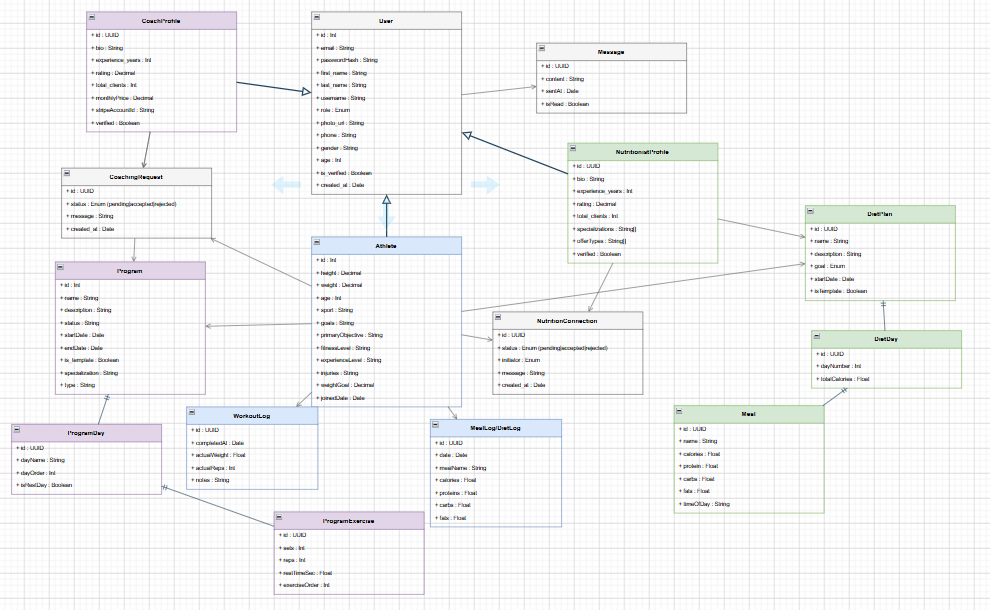
\includegraphics[width=1\textwidth]{diagrams/classe global.png}
\caption{Diagramme de classes global}
\end{figure}

\section{Conclusion}
Dans ce chapitre fondamental, nous avons traduit la vision globale du projet en spécifications techniques concrètes. La modélisation UML (Cas d'utilisation et Classes) nous a permis de structurer mentalement le comportement et les données de CoachingApp. La justification rigoureuse de notre pile technologique (Flutter, Angular, Node.js, PostgreSQL) a posé les fondations de l'architecture 3-Tiers robuste que nous avons décrite. À présent que le "Quoi" et le "Avec quoi" ont été fermement établis, les chapitres suivants seront dédiés au "Comment", en détaillant la réalisation technique de l'application à travers le déroulement des différents Sprints de développement.
